\chapter{Development Risk}
\label{ch:deve_risk}

It is important to assess the development risks associated with the various concepts as this gives important insight into the their feasibility. Development risks are the risks related to the development phase. Therefore, these are the risks of not being able to comply with the constraints, such as on time and money. In order to characterise the development risk associated with each concept, it is first necessary to identify a number of factors that are influential. These factors include:

\begin{enumerate}
    \item The level of feasibility of the concept. This depends on weather the concept has been proven and implemented before. 

    \item The level of complexity of component and elements contained in the concept. Does the concept contain systems or mechanisms that are not directly available at the moment, but require development or optimisation for this application? The required technology might still be in its infancy. Assessing this risk is thus of vital importance.
  
    \item The availability of knowledge or expertise related to a particular concept. This can be regarded as a development risk decreasing factor; the more available, the less risk there will be.
    
\end{enumerate}

\section{Concept Evaluation}

In the first subsection of this section the grading system will be elaborated on. the second subsection contains the grading table of the concepts with respect to development risk.

\subsection{Grading system} %maybe rephrase name
%These expected design obstacles can be expressed as risks that need to be assessed. 

A concept with a higher level of complexity has, by definition, less predictability. This means there is the risk that during the development unpredicted problems may show up; problems that cause the design to require more resources than prior foreseen. For instance, more time and money is needed to research certain unexpected phenomena and implement measures to counteract these.

What does this mean in practical terms for the case that a complex mechanism is incorporated in a design concept? In case the mechanism has not been used before, there is a substantial risk that the expected development resources needed will be more than prior estimated. This is due to the fact that there is no proof that the concept works. In the current concept selection, all the mechanism in the concepts do exist.  However, existing concepts might need optimisation for their application. A tandem rotating wing mechanism, for instance, has been used in aircraft design, but has seldom been implemented in a UAV application. Due to the level of complexity, which means higher uncertainty, this process might need more required resources as foreseen.

All the concepts will be analysed with regard to development risk in a qualitative way. For the quantitative approach a Technology Feasibility Scale (TFS) was created. This scale is inspired by the Technology Readiness Level Scale created by NASA\footnote{\url{https://www.nasa.gov/directorates/heo/scan/engineering/technology/txt_accordion1.html}, Accessed 22-05-2017}. By means of this TFS, a value can be attributed to the development risk of each concept.\\

\noindent The TFS, as portrayed in \autoref{fig:DRS}, has five different levels, labelled from A to E.

%no need for period in short itemise!
\begin{itemize}
    \item \textbf{A:} Commonly applied concept (0\% - 20\%)
    \item \textbf{B:} Concept with existing UAV applications (10\% - 40\%)
    \item \textbf{C:} Proven concept by means of working prototype (30\% - 60\%)
    \item \textbf{D:} Never applied, but theoretically feasible (50\% - 80\%)
    \item \textbf{E:} High risk that the concept is infeasible to develop (70\% - 100\%)
\end{itemize}

\begin{figure}[htb]
    \centering
    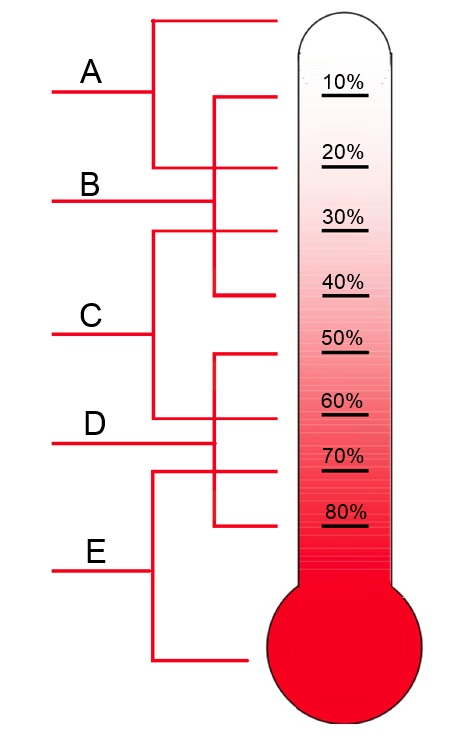
\includegraphics[width=.30\textwidth]{DevelopmentRisk/Figures/DRS.jpg}
    \caption{Technology Feasibility Scale}
    \label{fig:DRS}
\end{figure}

Next to the Technology Feasibility Scale, there are two other aspects that influence the total development risk. First, the level of complexity of the design; high complexity increases the development risk by an estimated percentage range of 0-20 percent. This value will be assigned to a concept based on the qualitative analysis, that can be found in \autoref{sec:qca}. The development risk is lowered if a knowledge source is available, which can assist the preventing of potential development stagnations. An example of this is the TU Delft tail sitter ATMOS, the expertise at the university decreases the development risk by an estimated percentage of 10 percent. 

\subsection{Grading of the concepts}

\autoref{tab:developmentrisk} shows the grading of the concepts. The percentages are shown in the different columns and by means of adding up, the development risk is obtained.

\begin{table}[H]
\caption{Concept Development Risk Grading}
\label{tab:developmentrisk}
\centering

\begin{tabular}{r|>{\centering}p{2.5cm}:>{\centering}p{2.5cm}:>{\centering}p{2.5cm}|c} 
\textbf{Concept \rotatebox{90}{\hspace{0.5cm}Criterion}} & \rotatebox{90}{\textbf{Feasibility [\%]}} & \rotatebox{90}{\textbf{Complexity [\%]}} & \rotatebox{90}{\textbf{Avail. Expertise [\%]}}  & \rotatebox{90}{\textbf{Dev. Risk [\%]}} 
    \\ \midrule

Tailsitter      & 25 & +10 & -10 & 25 
\\ \hdashline
Tandem          & 50 & +15 & 0 & 65 
\\ \hdashline
Prandtl Box     & 35 & +5 & -10 & 30 
\\ \hdashline
Tiltrotor       & 40 & +15 & 0 &  55
\\ \hdashline 
Winged Quad.    & 5 & 0 & 0 & 5
\\ \bottomrule
\end{tabular}

\end{table}


%%%%%
%Quality control Kelbey till here
%%%%%

\section{Qualitative Concept Analysis}
\label{sec:qca}
In this section, each concept will be analysed based on how much inherent development risk is present. Each concept will be analysed based on the grading system laid down in the previous section.

\subsection{Concept 1: The Tail sitter}
The Tailsitter is a proven concept; there are working prototypes and even some models available on the market. One can think about the ATMOS UAV\footnote{\url{http://www.atmosuav.com/}, Accessed 22-05-2017} and the DelftaCopter\footnote{\url{http://www.delftacopter.nl/delftacopter/}, Accessed 22-05-2017}. For this reason, this concept is classified as a category B on the Technology Feasibility Scale. 

There are no complex mechanism, like rotating parts, to be incorporated in the design that might induce any other development risk. However, there is some increase in risk due to the need for a complex control system in the transition phase from vertical to horizontal flight. This is included as a 10\% risk increase. For solutions to problems that occur, one of the existing designs can be consulted. Added to that is the fact that the TU Delft has a lot of expertise in the field of hybrid UAV Tailsitter concepts. This is included in the form of a development risk reduction of 10\%, which cancels out the 10\% increase caused by the control system. Due to the expertise and knowledge available at TU Delft, the development risk associated with designing the control system can be offset. 

\subsection{Concept 2: The Tandem}
This concept comprises three key elements which need to be examined when considering the development risks associated with it. 

The first element is the tandem wing configuration. Concepts and prototypes of hybrid UAVs using this wing configuration do exist; an example is the Airbus’s Quadcruiser UAV.  The second key element of this design is the use of four rotors for both VTOL and for horizontal flight. This is the most common configuration for VTOL UAVs because of the good stability and manoeuvrability this configuration offers. There is little development risk associated with utilising a quad-rotor.
The rotating wing Hybrid UAV concepts has been proven to be a feasible concept (The Greased Lightning GL-10\footnote{\url{https://www.nasa.gov/langley/ten-engine-electric-plane-completes-successful-flight-test}, Accessed 24-05-2017}). However, the rotating wing and the mechanics it introduces will cause a higher level of complexity. The level of complexity of the rotating wing is even considered higher than the level of complexity of just a tilt rotor \cite{princeton}. Like stated in the introduction of this chapter, extra complexity will increase the development risk. In this case, the net effect is an risk increase of 15\%.

So far as literature study goes, no commercially available UAV which resembles this concept was found. There is, however, one concept under development which does combines the three key elements. GH Craft, Japan is developing a tandem, rotating wing UAV demonstrating that this concept possesses some degree of feasibility\footnote{\url{http://www.ghcraft.com/QTW/QTW-UAS.htm}, Accessed 22-05-2017}. It is therefore classified as a Category C concept but towards the high risk end of the said category for the reasons mentioned above.

\subsection{Concept 3: The Prandtl Box}
Elements that are relevant to consider with regard to development risk are the rotating motors and the Prandtl wing box. The rotating motors contain mechanisms that introduces complexity to the design. There is the risk that the development of those systems to the point that they perform adequately might require more resources than foreseen. This is included in the grading as a risk increase of 5\%.

Although the Prandtl box concept is currently not used in general aviation, it is a proved concept. The AVY concept also incorporates the Prandtl wing box in their UAV design \footnote{\url{http://www.avy.eu/}, Accessed 11-05-2017}. This means that the development risks of this concept are limited; the chance that using this concept in the design will result in an unexpected resource requirements or even turns out to be unfeasible is unlikely. Due to the fact that AVY has a working prototype, and there are other Prandtl box configurations, this concept is classified as a Category C on the Technology Feasibility Scale. The value assigned to this concept is on the low end of this Category, namely 35\%.

\subsection{Concept 4: The Tiltrotor}
The Tiltrotor concept has been used before in both manned aerial vehicles and UAV applications. Aerial vehicles with a tiltrotor configuration are the V-22 Osprey and Bell Eagle Eye. Since this concept has been implemented successfully, The Tiltrotor is considered a category B on the Technology Feasibility Scale, but towards the high risk end of this category (namely 40 \%) because of the low number of tiltrotor UAVs on the market.                                   
The Tiltrotor concept presents a seemingly straightforward concept characterised by a conventional configuration with rotatable motors at the ends of the main wing. It seems that the complexity of this concept is quite low, but the opposite is true. 

Key to the success of this concept is a very advanced control system which must be meticulously developed and extensively tested. This control system is required to maintain controllability especially during the transition from vertical flight to horizontal flight as well as during hovering. The risk associated with not being able to develop an adequate control system capable of meeting the requirements is therefore large. Furthermore, an important factor in assessing the development risk is characterising the cost of development typical of such a design. The fact that this concept only has two rotors means that the controllability is substantially more difficult. Assuming that a control system capable of meeting the control requirements can be developed, substantial cost will be associated with developing it. The complexity of the control system translates into a large number of man-hours required for development and testing increasing the cost associated with the development. In the grading this is taken into account by a risk increase of 15\%.

In order to accomplish a successful design, thought needs to be given to what systems are necessary. The fact that there are only two rotors increases the required complexity of the design even further. In the event of one motor failing, the choice whether or not to include redundancy is an important factor in the level of development risk associated with this concept. If a redundant system is chosen, a complicated drive axis system would be required such that each motor can drive the other in the event of a failure. The development risk associated with this is large. 

\subsection{Concept 5: The Winged Quadcopter}
The Winged Quadcopter merges a conventional configuration airplane with a quadcopter. This is the most basic hybrid UAV concept and as a result has very little development risk. Due to the conventionality of this concept, it is classified as a category A on the Technology Feasibility Scale and has a assigned percentage of just 5\%.

There are many Hybrid UAVs on the market that utilise this or a very similar concept. This is an indication of the technical feasibility as well as the ease of development associated with this concept. Complexity is introduced by adding the capability of rotating the rotors in order to make use of them in both flight regimes (vertical \& horizontal). This increases not only the mechanical complexity but also the complexity of the control system and thus increasing the development risk.

Nevertheless, conventional configuration UAVs with four tilt rotors are commercially available. Quantum Systems develops and sells such a concept proving the technical and commercial feasibility of such a concept\footnote{\url{https://www.quantum-systems.com/}, Accessed 24-05-2017}. This indicates that the development risk linked to concept 5 is moderate to low and can thus be quantified so low that it can be neglected.

